\chapter{Algorithmen} \label{algorithmen}

% Beispiel für Glossar/Abkürzungen
% Der \gls{accesspoint} sendet die \gls{bssid} und die \gls{ssid}, damit Geräte, wie eine \gls{vm}, sich verbinden können. Algorithmen wie \gls{knn} und \gls{svm} können in einer \gls{api} implementiert werden, um die Datenverarbeitung zu optimieren.


% \begin{table}[h]
%     \centering
%     \begin{tabularx}{\textwidth}{|X|X|X|X|X|}
%         \hline
%         Router & Raum 1      & Raum 2      & Raum 3     & Unbekannt (1) \\ \hline
%         1      & -73.67 dBm  & -91.12 dBm  & -69.37 dBm & -73.51 dBm    \\ \hline
%         2      & -104.99 dBm & -64.47 dBm  & -89.65 dBm & -103.41 dBm   \\ \hline
%         3      & -67.03 dBm  & -105.38 dBm & -88.40 dBm & -70.35 dBm    \\ \hline
%     \end{tabularx}
%     \caption{RSSI-Werte für die drei Router und die Räume}
%     \label{tab:rssi_values}
% \end{table}

Für die Vorhersage einer Position bei der Indoor-Ortung mittels WiFi-Fingerprints können verschiedene Algorithmen verwendet werden. Es wurde sich dafür entschieden in dieser Arbeit die Modelle K-Nearest Neighbors (KNN), Support Vector Machines (SVM) und Random Forest zu verwenden, da diese Modelle bereits in anderen Untersuchungen gute Ergebnisse erzielen konnten.\myfootcite{Han2018WirelessFingerprint}{S. 3}\textsuperscript{,}\myfootcite{Rezgui2017NormalizedSVM}{S. 13}

Im Folgenden werden die drei verwendeten Algorithmen detailliert beschrieben und für eine bessere Verständlichkeit anhand eines Beispiels, welches in Tabelle \ref{tab:trainingsdaten} dargestellt ist, erläutert. In diesem Beispiel wurden die RSSI-Werte von sechs Messungen in drei verschiedenen Räumen sowie drei Access Points simuliert. In der Tabelle \ref{tab:testdaten} sind die RSSI-Werte von einer Messung in einem unbekannten Raum, für die eine Vorhersage gemacht werden soll, aufgeführt. Die in den Tabellen dargestellten Werte basieren nicht auf realen Messungen und sind hypothetische Beispielwerte, welche gewählt wurden, um die Funktionsweise der Algorithmen zu veranschaulichen und die Nachvollziehbarkeit der Berechnungen zu erleichtern.

\begin{table}[h]
    \centering
    \begin{tabularx}{\textwidth}{|X|X|X|X|X|}
        \hline
        Messung & Raum & AP1 & AP2 & AP3 \\ \hline
        1 & A & -45 dBm & -60 dBm & -70 dBm \\ \hline
        2 & A & -46 dBm & -61 dBm & -71 dBm \\ \hline
        3 & B & -55 dBm & -65 dBm & -75 dBm \\ \hline
        4 & B & -54 dBm & -66 dBm & -74 dBm \\ \hline
        5 & C & -50 dBm & -70 dBm & -80 dBm \\ \hline
        6 & C & -51 dBm & -69 dBm & -79 dBm \\ \hline
    \end{tabularx}
    \caption{Beispielwerte von WiFi-Fingerprints aus der Offline-Phase}
    \label{tab:trainingsdaten}
\end{table}

\begin{table}[h]
    \centering
    \begin{tabularx}{\textwidth}{|X|X|X|X|X|}
        \hline
        Messung & Raum & AP1 & AP2 & AP3 \\ \hline
        - & - & -52 dBm & -68 dBm & -78 dBm \\ \hline
    \end{tabularx}
    \caption{Beispielwerte eines WiFi-Fingerprints aus der Online-Phase}
    \label{tab:testdaten}
\end{table}


% \mycitefoot{Shang2022WiFiFingerprinting}
% \myfootcite{masoud2022access}{S. 5464}

% \paragraph{Quellen für Auswahl}

% \begin{itemize}
%     \item https://ar5iv.labs.arxiv.org/html/2111.14281 -> KNN, SVM % Hoang2021PassiveLocalization
%     \item A Wireless Fingerprint Location Method Based on Target Tracking (Kapitel 3, Seite 3) -> KNN, SVM, Random Forest % Han2018WirelessFingerprint
%     \item https://onlinelibrary.wiley.com/doi/full/10.1155/2017/6268797 Name: An Efficient Normalized Rank Based SVM for Room Level Indoor WiFi Localization with Diverse Devices -> KNN, SVM, Random Forest. In Table 2 stehen die Genauigkeiten der Algorithmen S. 13% Rezgui2017NormalizedSVM
% \end{itemize}

\section{K-Nearest Neighbors (KNN)}

% \textbf{Quellen:} \\
% \href{https://www.ibm.com/de-de/topics/knn}{Quelle 1: https://www.ibm.com/de-de/topics/knn} \\ % ibmknearestNeighbors
% Quelle 4: Comprehensive analysis of distance and similarity measures for Wi-Fi fingerprinting indoor positioning systems \\ % TorresSospedra2015WiFi
% Quelle 5: Hechenbichler, Schliep: - Weighted k-Nearest-Neighbor Techniques and Ordinal Classification % Hechenbichler2004WeightedKNN

% \subsection{Algorithmusbeschreibung}

Der \gls{knn} Algorithmus ist ein überwachter Lernalgorithmus, der auf dem Konzept der Nähe basiert und zur Lösung von Klassifikations- und Regressionsproblemen verwendet werden kann. Der Algorithmus funktioniert so, dass ein Datenpunkt mit den vorhandenen Datenpunkten in den Trainingsdaten verglichen wird und die Distanz zu jedem Datenpunkt berechnet wird. Dabei wird die Distanz der einzelnen Features, welche in dem Fall der Indoor-Ortung die RSSI-Werte der Access Points sind, berechnet und aufsummiert. Basierend auf diesen Distanzen werden die \( k \)-Datenpunkte ausgewählt, die den kleinsten Abstand haben. Aus diesen \( k \)-Datenpunkten wird dann die Klasse vorhergesagt, die am häufigsten vertreten ist. Bei der Indoor-Ortung entsprechen die Klassen den verschiedenen Räumen.\mycitefoot{ibmknearestNeighbors}

\subsection{Distanzmetriken}
Für die Berechnung der Distanzen können verschiedene Distanzmetriken verwendet werden. Die am häufigsten verwendete Distanzmetrik ist der euklidische Abstand. Bei der euklidischen Distanz wird das Quadrat der Abstände zwischen zwei Werten gebildet, über alle Wertepaare aufsummiert und abschließend die Quadratwurzel dieser Summe gezogen (siehe Gleichung \ref{eq:euclidean}).\mycitefoot{ibmknearestNeighbors}

\begin{equation}
    \label{eq:euclidean}
    \text{distance}_{\text{euclidean}}(P, Q) = \sqrt{\sum_{i=1}^{d} (P_i - Q_i)^2}
\end{equation}

Bei der Sørensen-Distanzfunktion werden die Beträge der Abstände der Datenpunkte aufsummiert und durch die Summe der addierten Wertepaare geteilt (siehe Gleichung \ref{eq:sorensen}). Grund für die Wahl dieser beiden Metriken sind die Ergebnisse der Arbeit \textit{Comprehensive analysis of distance and similarity measures for Wi-Fi fingerprinting indoor positioning systems}, welche mit der Sørensen Distanz gute Ergebnisse erzielen konnte und die Tatsache, dass die euklidische Distanz weit verbreitet ist und der bisherigen Implementierung in der \textit{BVG Detection} App entspricht.\mycitefoot{TorresSospedra2015WiFi}

\begin{equation}
    \label{eq:sorensen}
    \text{distance}_{\text{sorensen}}(P, Q) = \frac{\sum_{i=1}^{d} |P_i - Q_i|}{\sum_{i=1}^{d} (P_i + Q_i)}
\end{equation}

Um die Unterschiede dieser beiden Metriken zu veranschaulichen, wurden die Distanzen für alle möglichen Wertepaare zwischen 0\,dBm und -100\,dBm berechnet und in Abbildung \ref{fig:distance_metrics_heatmaps} dargestellt. Wie zu erkennen ist, ist bei der euklidischen Distanz ausschließlich die Differenz der beiden Werte ausschlaggebend, was sich anhand der symmetrischen Anordnung der Werte in der Heatmap entlang der Geraden, die durch die Punkte (0\,dBm, -100\,dBm) und (-100\,dBm, 0\,dBm) sowie (0\,dBm, 0\,dBm) und (-100\,dBm, -100\,dBm) verläuft, zeigt. Im Gegensatz dazu ist die Sørensen-Distanz sowohl von der Differenz als auch von der Summe der beiden Werte abhängig, was sich durch das Fehlen einer Symmetrie entlang der genannten Geraden zwischen den Punkten (0\,dBm, -100\,dBm) und (-100\,dBm, 0\,dBm) zeigt. Bei kleineren Werten ist ein größerer Abstand erforderlich, um die gleiche Distanz wie bei größeren Werten zu erreichen. Dies könnte sich vorteilhaft auf die Indoor-Ortung auswirken, da die RSSI-Werte nicht linear mit der Entfernung korrelieren, wie in Abbildung \ref{fig:plot_rssi_distance} dargestellt ist.


% Um dies zu verdeutlichen, betrachten wir die Berechnung der Distanzen für zwei Beispielwertepaare:

% Gegeben:
% \begin{itemize}
%     \item Wertepaar 1: \( P = -30 \, \text{dBm} \), \( Q = -40 \, \text{dBm} \)
%     \item Wertepaar 2: \( P = -70 \, \text{dBm} \), \( Q = -80 \, \text{dBm} \)
% \end{itemize}

% \begin{table}[H]
%     \centering
%     \begin{tabular}{|c|c|c|}
%         \hline
%         Wertepaar                                & Sørensen-Dice Distanz & Euklidische Distanz \\
%         \hline
%         \(-30 \, \text{dBm}, -40 \, \text{dBm}\) & \(-0.142857\)         & \(10\)              \\
%         \(-70 \, \text{dBm}, -80 \, \text{dBm}\) & \(-0.066667\)         & \(10\)              \\
%         \hline
%     \end{tabular}
%     \caption{Berechnete Distanzen für die gegebenen Wertepaare}
%     \label{tab:distance_results}
% \end{table}

% Um das zu verdeutlichen wurden die Distanzen für beide Metriken anhand der Beispielwerte berechnet wie in Tabelle \ref{tab:distanzen} dargestellt.

Für die Beispielwerte ergeben sich dadurch folgende Distanzen

Die sich für die Beispielwerte aus Tabelle \ref{tab:trainingsdaten} ergebenen Distanzen sind in Tabelle \ref{tab:distanzen} dargestellt.

\begin{table}[h]
    \centering
    \begin{tabularx}{\textwidth}{|X|X|X|X|}
        \hline
        Messung & Raum & Euklidische Distanz & Sørensen Distanz \\ \hline
        1 & A & 11.0 & 0.084 \\ \hline
        2 & A & 9.8 & 0.077 \\ \hline
        3 & B & 5.2 & 0.034 \\ \hline
        4 & B & 4.5 & 0.030 \\ \hline
        5 & C & 3.5 & 0.020 \\ \hline
        6 & C & 2.6 & 0.015 \\ \hline
    \end{tabularx}
    \caption{Berechnete Distanzen der Beispieldaten}
    \label{tab:distanzen}
\end{table}

\begin{figure}[H]
    \centering
    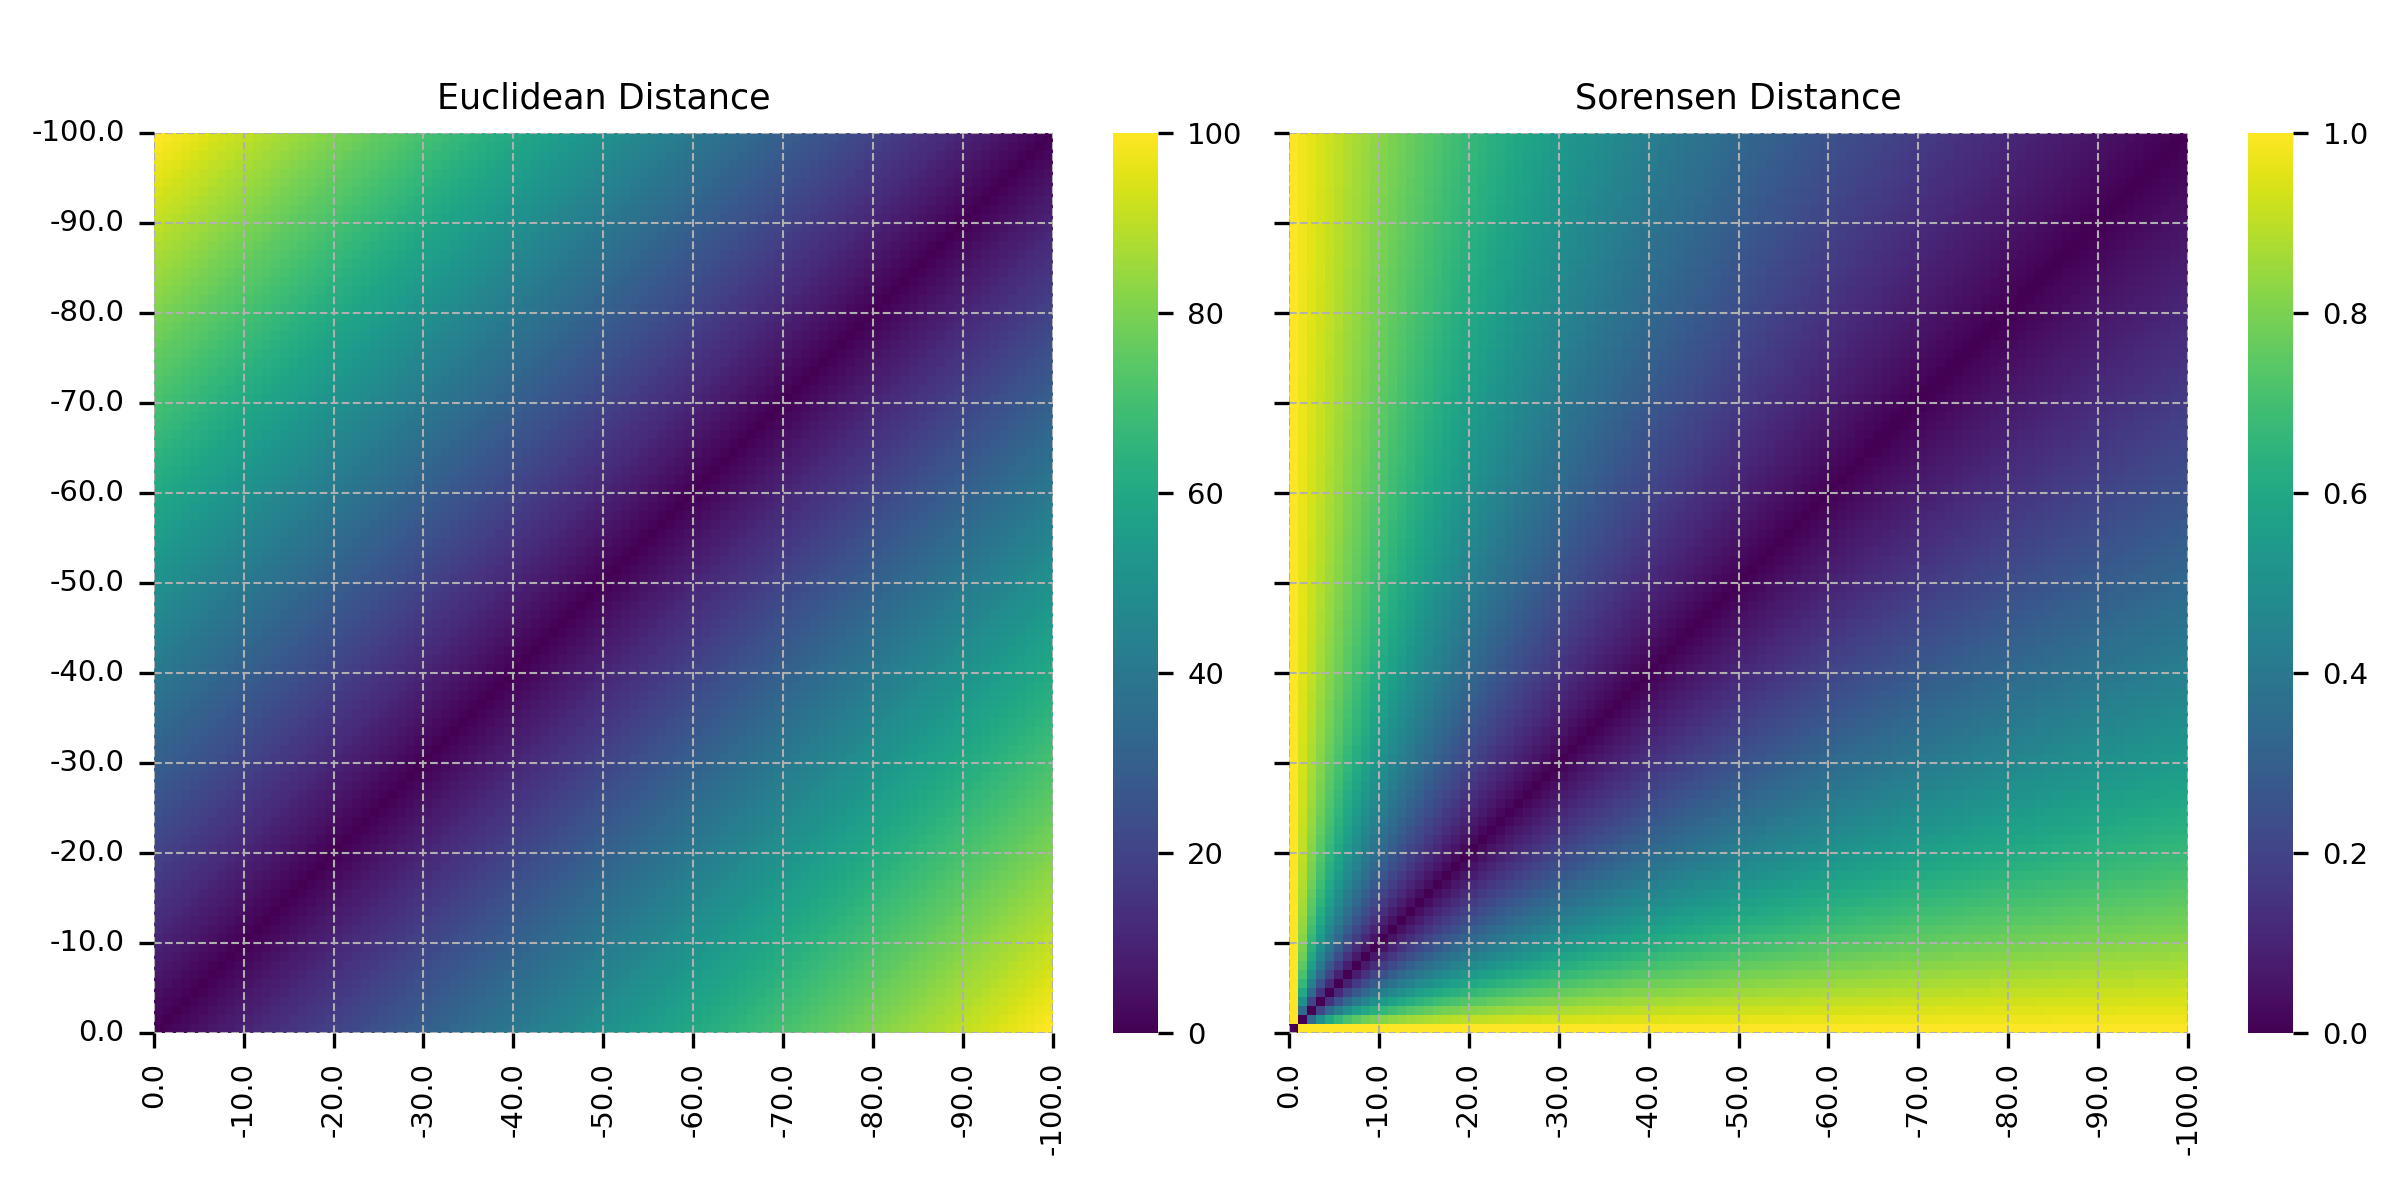
\includegraphics[width=0.8\textwidth]{images/plot_euclidean_vs_sorensen.png}
    \caption{Vergleich der Distanzmetriken Euklidisch und Sørensen}
    \label{fig:distance_metrics_heatmaps}
\end{figure}

\subsection{Anzahl der Nachbarn}

Der Parameter \( k \) legt fest, wie viele nächste Nachbarn für die Klassifizierung berücksichtigt werden. Kleine Werte für \( k \) können zu hoher Varianz und geringer Verzerrung führen, während größere Werte die Varianz verringern, jedoch die Verzerrung erhöhen. Die Wahl des optimalen \( k \)-Werts hängt stark von den vorhandenen Trainingsdaten ab. Bei Daten mit Ausreißern oder Rauschen empfiehlt es sich, höhere \( k \)-Werte zu wählen, da diese in solchen Fällen bessere Ergebnisse liefern. Um Gleichstände bei dem Mehrheitsvotum zu vermeiden, sollten ungerade Werte für \( k \) bevorzugt werden.\mycitefoot{ibmknearestNeighbors}

Bei einem Wert von \( k = 3 \) würden für beide Distanzen in dem Beispiel die Werte der vierten, fünften und sechsten Messung für die Vorhersage verwendet werden, da für diese drei Messungen die Distanzen am geringsten sind (siehe Tabelle \ref{tab:distanzen}) und das Modell würde Raum C vorhersagen, da dieser unter den drei Messungen am häufigsten vertreten ist.

\subsection{Gewichtung}

Der \gls{knn}-Algorithmus kann erweitert werden, indem die Distanzen der \( k \) nächsten Nachbarn nach ihrer Berechnung gewichtet werden. Hierfür stehen verschiedene Gewichtungsfunktionen, wie zum Beispiel der Inversions-Kernel oder der Gauss-Kernel, zur Verfügung. Für Vorhersage unter Verwendung einer Gewichtungsfunktion, werden die Distanzen der \( k \) nächsten Nachbarn nach ihrer Berechnung in die Gewichtungsfunktion eingesetzt, für jede vertretene Klasse aufsummiert und es wird die Klasse mit dem größten Gewicht ausgewählt. Dadurch hat neben der relativen Häufigkeit der Klassen auch die Distanz der Nachbarn einen Einfluss auf die Klassifikation und es ist möglich eine nicht optimale Wahl des Parameters \( k \) auszugleichen.\myfootcite{Hechenbichler2004WeightedKNN}{S. 6}

In dieser Arbeit wurde sich dafür entschieden den Inversions-Kernel zu verwenden, da für die Implementierung des \gls{knn}-Algorithmus die Bibliothek \textit{scikit-learn} verwendet wird und der Inversions-Kernel der Standardgewichtungsfunktion dieser entspricht. Zudem hat die Wahl der Gewichtungsfunktion laut dem Paper \textit{Weighted k-Nearest-Neighbor Techniques and Ordinal Classification} in der Regel keinen entscheidenden Einfluss auf die Genauigkeit der Klassifikation.\myfootcite{Hechenbichler2004WeightedKNN}{S. 6}\textsuperscript{,}\mycitefoot{scikitlearnKNeighborsRegressor}

Die Gewichtungsfunktion des Inversions-Kernels ist gegeben durch:

\begin{equation}
    \label{eq:inversion}
    K(d) = \frac{1}{|d|}
\end{equation}

wobei \( d \) die Distanz darstellt. 

% Quelle für scikit-learn https://scikit-learn.org/stable/modules/generated/sklearn.neighbors.KNeighborsRegressor.html#sklearn.neighbors.KNeighborsRegressor

% Ein Vorteil dieser Gewichtung ist, dass so eine schlechte Wahl des Parameters k wieder ausgeglichen werden kann, da bei einem zu großen Wert für k 

% Wahl der Gewichtungsfunktion nicht sehr ausschlaggebend (Quelle 5, Seite 5, "But from experience the choice of a special kernel (apart from the special case of the rectangular kernel, that gives equal weights to all neighbors) is not crucial.")

\begin{table}[h]
    \centering
    \begin{tabularx}{\textwidth}{|X|X|X|X|}
        \hline
        Raum & Gewicht (Euklidisch) & Gewicht (Sørensen) \\ \hline
        C & 0,671 (0,385 + 0,286) & 116,667 (66,667 + 50) \\ \hline
        B & 0.222 & 33.333 \\ \hline
    \end{tabularx}
    \caption{Gewichtete Distanzen der drei nächstgelegenen Trainingsdaten}
    \label{tab:gewichtete_distanzen}
\end{table}

Unter Verwendung der Gewichtungsfunktion des Inversions-Kernels ergeben sich für das Beispiel die in Tabelle \ref{tab:gewichtete_distanzen} dargestellten gewichteten Distanzen und das Modell würde Raum C vorhersagen.

Für die detaillierten Untersuchungen in Kapitel \ref{untersuchungen} wurde sich dafür entscheiden den \gls{knn}-Algorithmus ohne Gewichtungsfunktion (\texttt{weights = uniform}) und mit Gewichtungsfunktion (\texttt{weights = distance}) zu vergleichen, um zu untersuchen, ob die Gewichtungsfunktion die Genauigkeit der Klassifikation verbessern kann.

\section{Support Vector Machines (SVM)}


% In Abbildung \ref{fig:myplot_7_svm} ist ein SVM dargestellt.

% \begin{figure}[H]
%     \centering
%     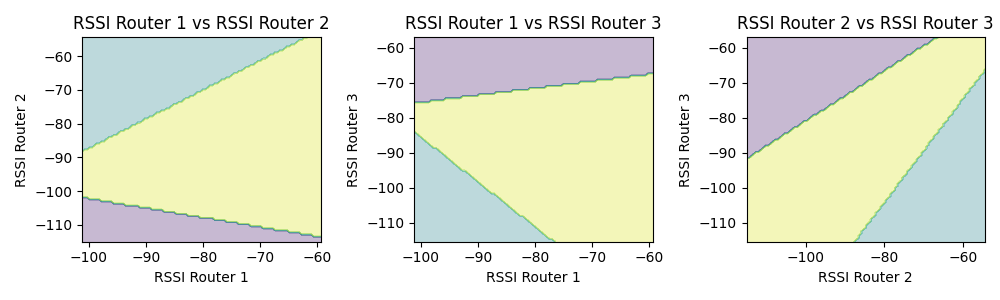
\includegraphics[width=0.8\textwidth]{images/myplot_7_svm.png}
%     \caption{SVM}
%     \label{fig:myplot_7_svm}
% \end{figure}

% \textbf{Quellen:} \\
% \href{https://www.bigdata-insider.de/was-ist-eine-support-vector-machine-a-880134}{Quelle 6: https://www.bigdata-insider.de/was-ist-eine-support-vector-machine-a-880134} \\ % bigdatainsiderEineSupport
% \href{https://www.ibm.com/topics/support-vector-machine}{Quelle 7: https://www.ibm.com/topics/support-vector-machine} \\ % ibmWhatSupport
% \href{https://wires.onlinelibrary.wiley.com/doi/full/10.1002/wics.49}{Quelle 8: https://wires.onlinelibrary.wiley.com/doi/full/10.1002/wics.49} % Mammone2009SVM


% Quelle warum gerade RBF: An Indoor Localization of WiFi Based on Support Vector Machines

% \subsection{Algorithmusbeschreibung}

Der Support Vector Machine (SVM) Algorithmus ist ein maschineller Lernalgorithmus, der für die Klassifizierung von Daten verwendet werden kann. Die Klassifizierung erfolgt, indem versucht wird die optimale Trennlinie – die sogenannte Hyperebene – zwischen den Datenpunkten zu finden. Die Hyperebene wird dabei so positioniert, dass der Abstand zwischen den Datenpunkten der beiden Klassen maximiert wird. In einem Beispiel mit zwei Merkmalen, wie in Abbildung \ref{fig:svm_hyperplane}, lassen sich die Datenpunkte beider Klassen in einem zweidimensionalen Koordinatensystem als Punkte darstellen und die Hyperebene als Linie. 

Der \gls{svm} Algorithmus ist auch in der Lage mit mehr als zwei Merkmalen zu arbeiten, indem versucht wird eine Hyperebene in einem mehrdimensionalen Raum, welche die Datenpunkte der verschiedenen Klassen voneinander trennt, zu finden.\mycitefoot{ibmWhatSupport}

\begin{figure}[H]
    \centering
    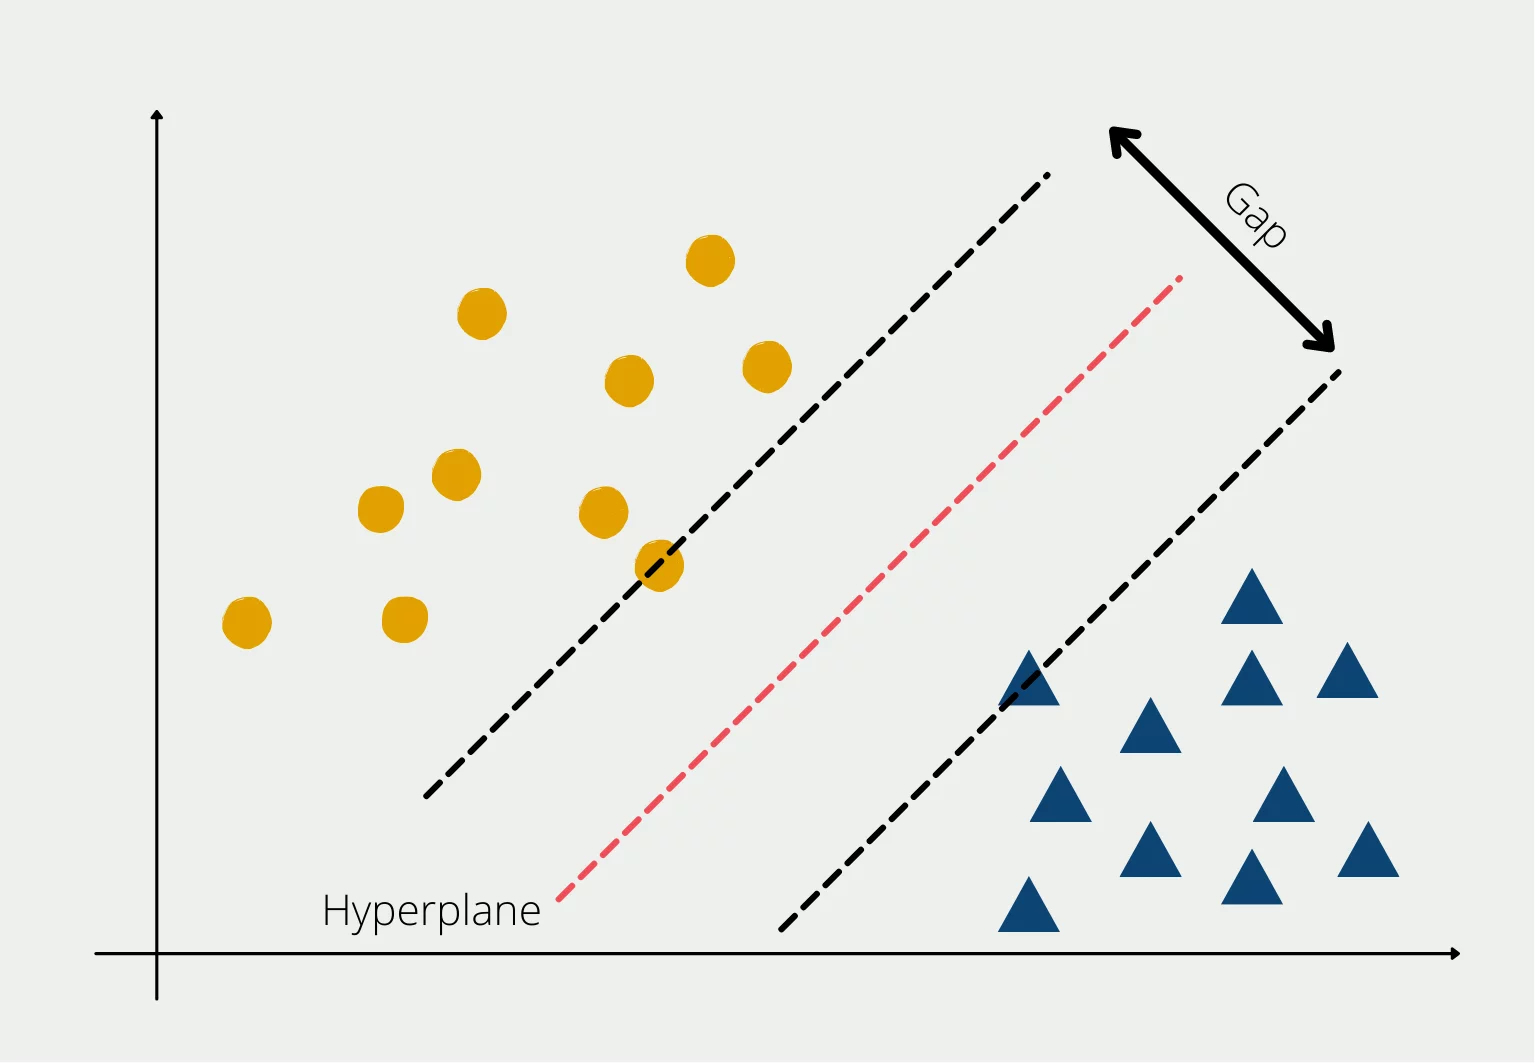
\includegraphics[width=0.4\textwidth]{images/source_svm.png}
    \caption{Darstellung einer Hyperebene in einem \gls{svm} mit zwei Features (Bildquelle: \citeauthor{databasecampSupportVector} \citeyear{databasecampSupportVector})}
    \label{fig:svm_hyperplane}
\end{figure}

\subsection{Auswahl des Kernels}

In Abbildung \ref{fig:svm_hyperplane} konnten die Daten durch eine Gerade getrennt werden, weswegen ein \gls{svm} mit einem linearen Kernel verwendet werden konnte. Sollten die Daten nicht linear trennbar sein - wie in Abbildung \ref{fig:source_svm_rbf} - sollte ein anderer Kernel verwendet werden. In diesen Fällen wird zuerst die Kernel-Methode angewendet, welche die Daten in einen höherdimensionalen Raum transformiert, und anschließend wird versucht die Daten in diesem Raum linear zu trennen.\mycitefoot{ibmWhatSupport}

In dieser Arbeit wurde sich dafür entschieden, den linearen Kernel mit einem nicht linearen Kernel zu vergleichen. Für das nicht lineare \gls{svm} wurde der RBF-Kernel gewählt, da in der Arbeit \textit{Device-Free Presence Detection and Localization With SVM and CSI Fingerprinting} mit diesem Kernel die besten Ergebnisse unter den nicht linearen SVMs erzielt werden konnten.\mycitefoot{ibmWhatSupport}

\begin{figure}[H]
    \centering
    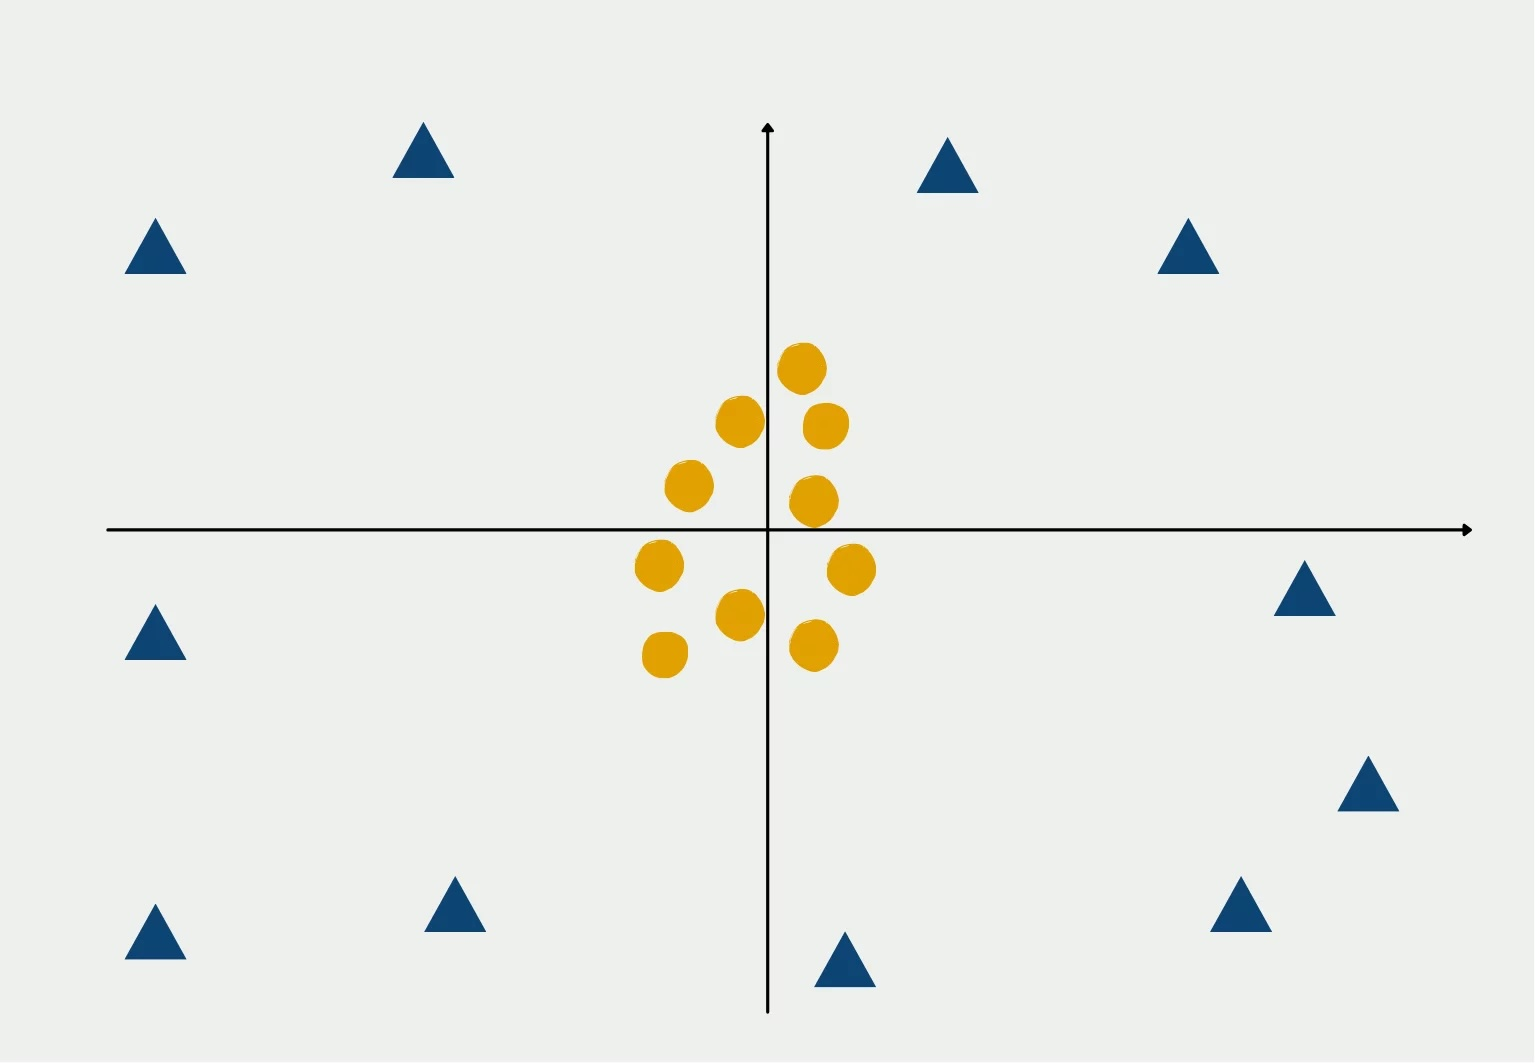
\includegraphics[width=0.4\textwidth]{images/source_svm_rbf.png}
    \caption{Darstellung von nicht linear trennbaren Daten in einem \gls{svm} (Bildquelle: \citeauthor{databasecampSupportVector} \citeyear{databasecampSupportVector})}
    \label{fig:source_svm_rbf}
\end{figure}

\subsection{Regularisierungsparameter C und Kernel-Parameter \texttt{gamma}}

% TODO: Margin erklären -> bereich in dem die Hyperebene liegt und bessere Bilder (Dort steht Gap...)

Der \gls{svm} Algorithmus kann über den Regularisierungsparameter C und den Kernel-Parameter \texttt{gamma} konfiguriert werden. Der Regularisierungsparameter C legt dabei fest, wie groß der Bereich ist, in dem die Hyperebene liegt. Also der Abstand zwischen den beiden schwarzen Linien in Abbildung \ref{fig:svm_hyperplane}. Je kleiner der Wert ist, desto größer ist der Abstand. Größere Werte für C können dazu führen, dass das Modell die Trainingsdaten gut klassifizieren kann, jedoch kann das auch dazu führen, dass das Modell fehleranfälliger bei der Klassifikation neuer Daten ist.\mycitefoot{baeldungParameterSupport}

Der Kernel-Parameter \texttt{gamma} kann nur für nicht lineare \gls{svm}-Modelle verwendet werden und legt fest, wie groß der Einfluss eines einzelnen Trainingsbeispiels bei der Berechnung der Hyperebene ist. Bei einem großen Wert für \texttt{gamma} ist der Einfluss eines einzelnen Trainingsbeispiels gering und es kann zum Overfitting. Dies bedeutet das dass Modell die Trainingsdaten zu stark berücksichtigt und neue Daten nicht so gut klassifizieren kann. Ein kleiner Wert für \texttt{gamma} kann dazu führen, dass das Modell zu stark vereinfacht wird und es zum Underfitting kommt.\mycitefoot{geeksforgeeksGammaParameter}

% Quelle für die Auswahl der Parameter Werte: Semi-Supervised Classification by Low Density Separation

\section{Random Forest}

% Gute quelle: WiFi Indoor Localization with CSI Fingerprinting-Based Random Forest -> Wie wichtig ist welcher Hyperparameter? % Wang2018WiFiLocalization

% In Abbildung \ref{fig:myplot_7_rf} ist ein Entscheidungsbaum dargestellt.

% \begin{figure}[H]
%     \centering
%     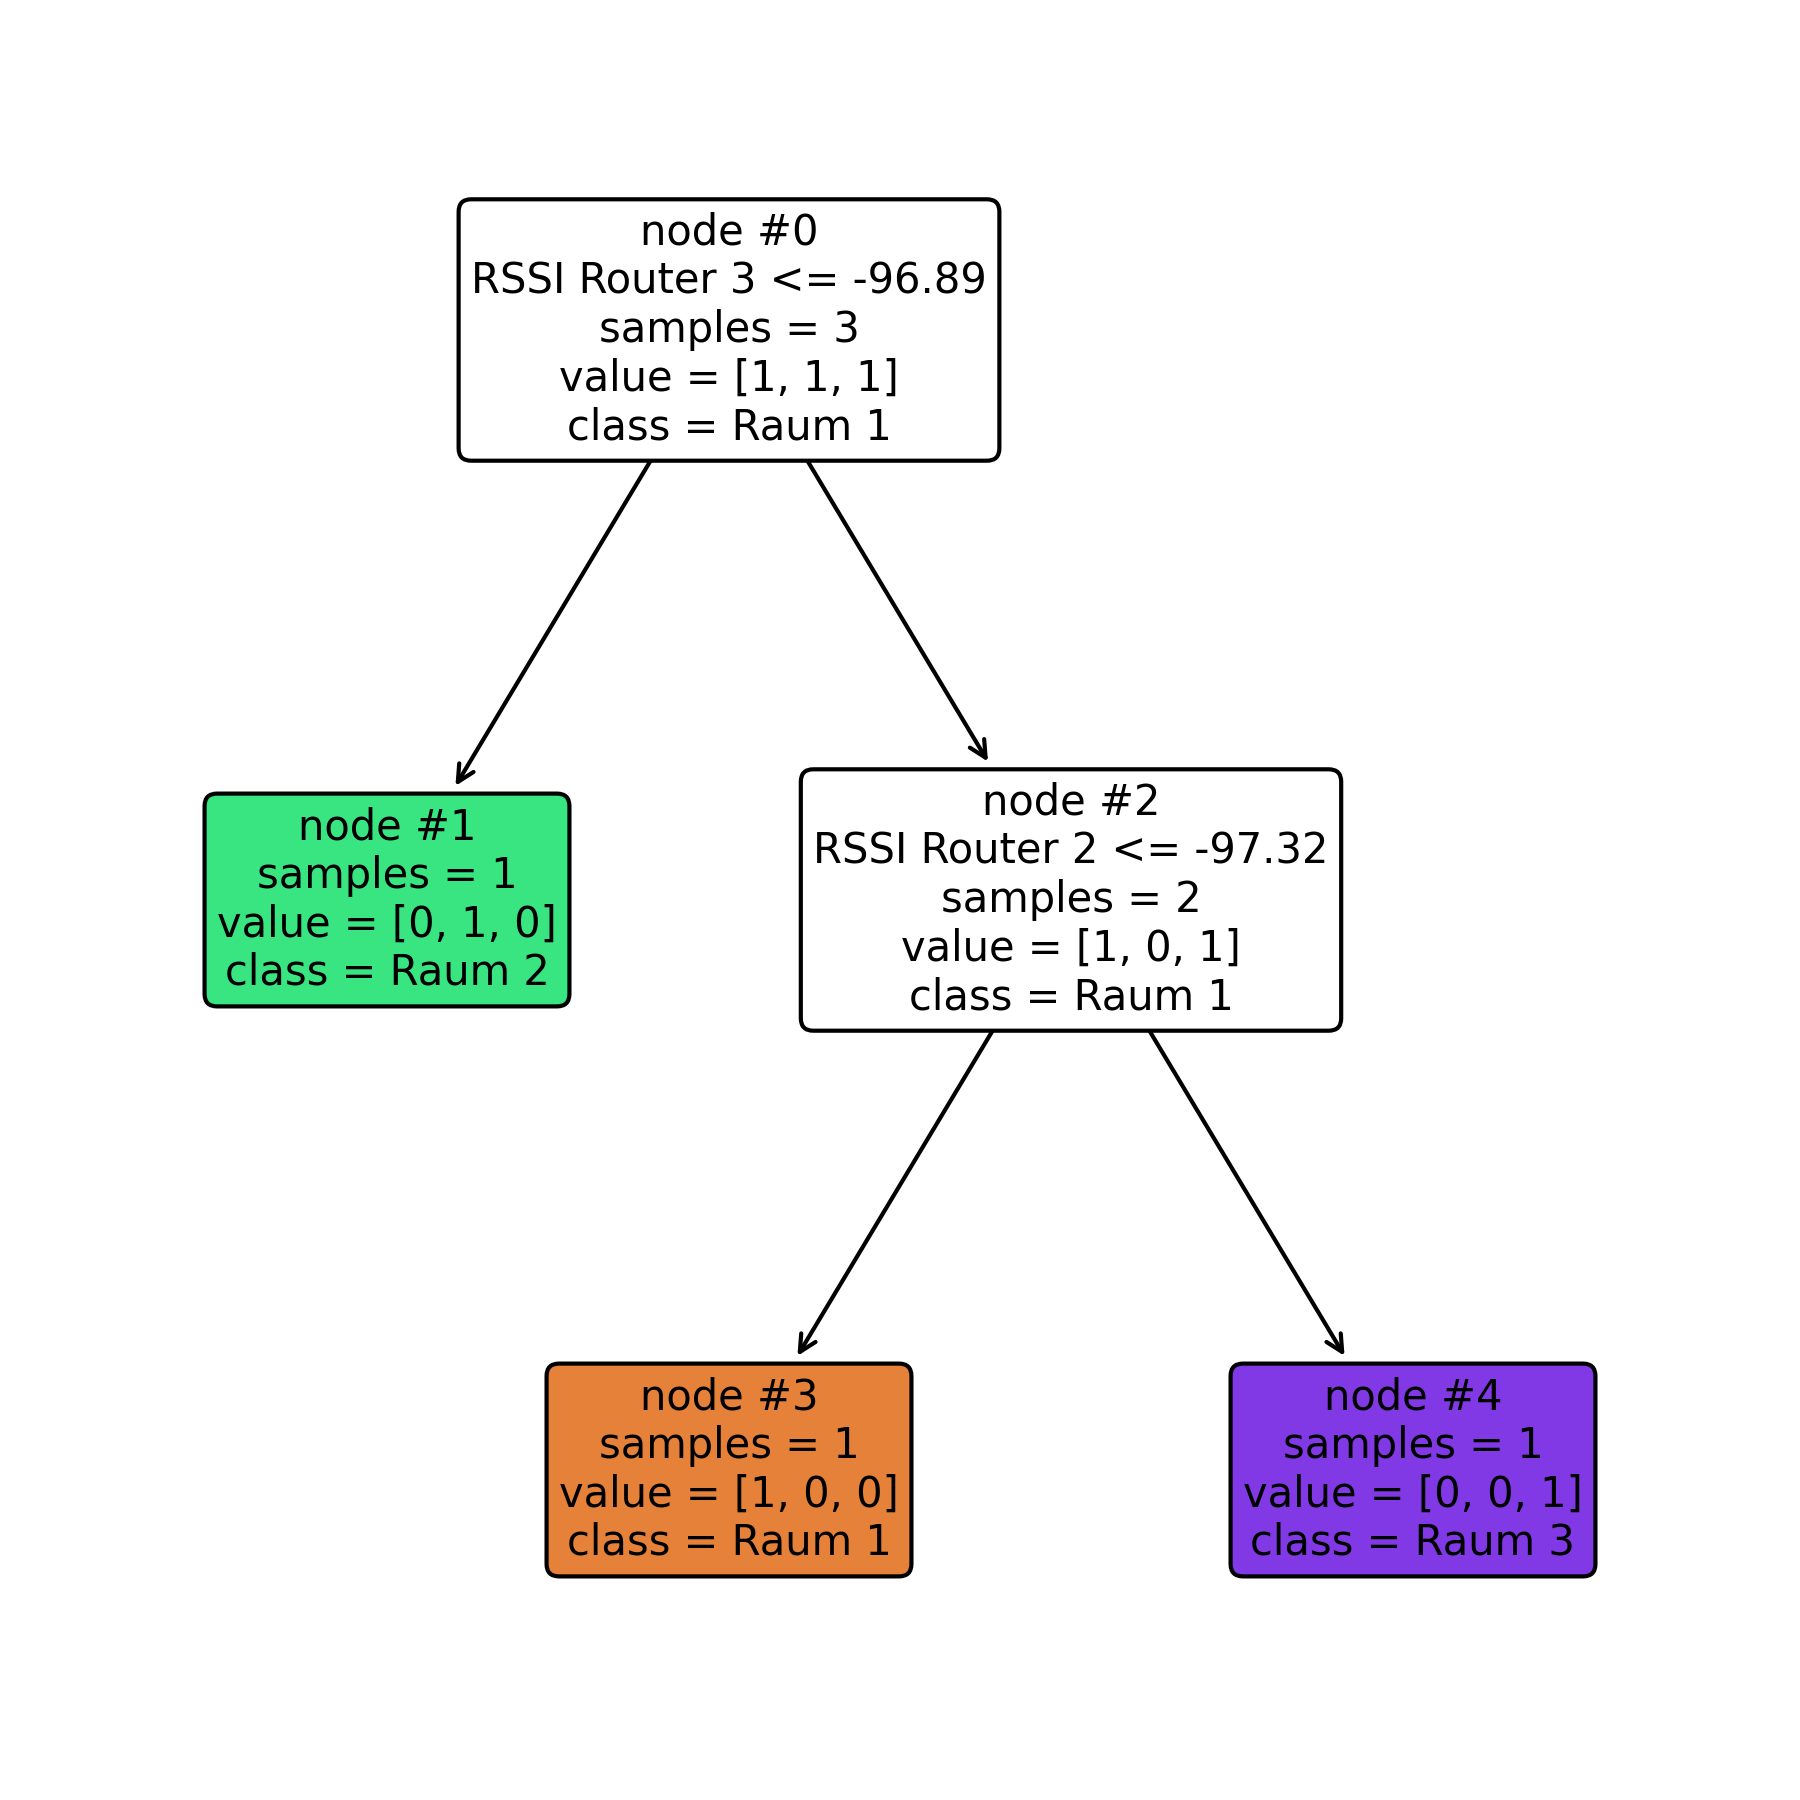
\includegraphics[width=0.8\textwidth]{images/myplot_7_rf.png}
%     \caption{Distance vs. Uniform weights}
%     \label{fig:myplot_7_rf}
% \end{figure}

% \textbf{Quelle:} \\
% \href{https://builtin.com/data-science/random-forest-algorithm}{Quelle 9: https://builtin.com/data-science/random-forest-algorithm} % builtinRandomForest

% \subsection{Algorithmusbeschreibung}

Der Random Forest-Algorithmus ist Lernalgorithmus der zur Klassifizierung verwendet werden kann. Dabei basiert die Vorhersage auf einer Vielzahl von Entscheidungsbäumen, die jeweils eine eigene Vorhersage treffen. Ein Entscheidungsbaum ist ein Modell, das Entscheidungen durch eine Abfolge von Wahl/Falsch-Abfragen trifft, die sich aus den Merkmalen der Daten ableiten. An jedem Knotenpunkt des Baumes wird eine Entscheidung basierend auf einem einzelnen Merkmal getroffen und am Ende eines jeden Entscheidungsbaums erfolgt eine Vorhersage. 

Für jeden Entscheidungsbaum im Random Forest wird eine zufällige Teilmenge der Trainingsdaten verwendet und die endgültige Vorhersage des Random Forests Modells ergibt sich aus einem Mehrheitsvotum der individuellen Entscheidungsbäume.\mycitefoot{builtinRandomForest}

Laut der Studie \textit{WiFi Indoor Localization with CSI Fingerprinting-Based Random Forest} sind die einflussreichsten Parameter des Random Forest Algorithmus die maximale Tiefe der Bäume (\texttt{max\_depth}), die Anzahl der Entscheidungsbäume (\texttt{n\_estimators}) sowie die maximale Anzahl der betrachteten Features (\texttt{max\_features}). Aus diesem Grund werden in dieser Arbeit diese Parameter in Bezug auf die Genauigkeit bei der Vorhersage untersucht.\myfootcite{Wang2018WiFiLocalization}{S. 18}

In Abbildung \ref{fig:random_forest} ist ein Entscheidungsbaum dargestellt, welcher mit Hilfe der Beispieldaten aus Tabelle \ref{tab:trainingsdaten} erstellt wurde und für die Daten aus Tabelle \ref{tab:testdaten} Raum C vorhersagen würde.

\begin{figure}[H]
    \centering
    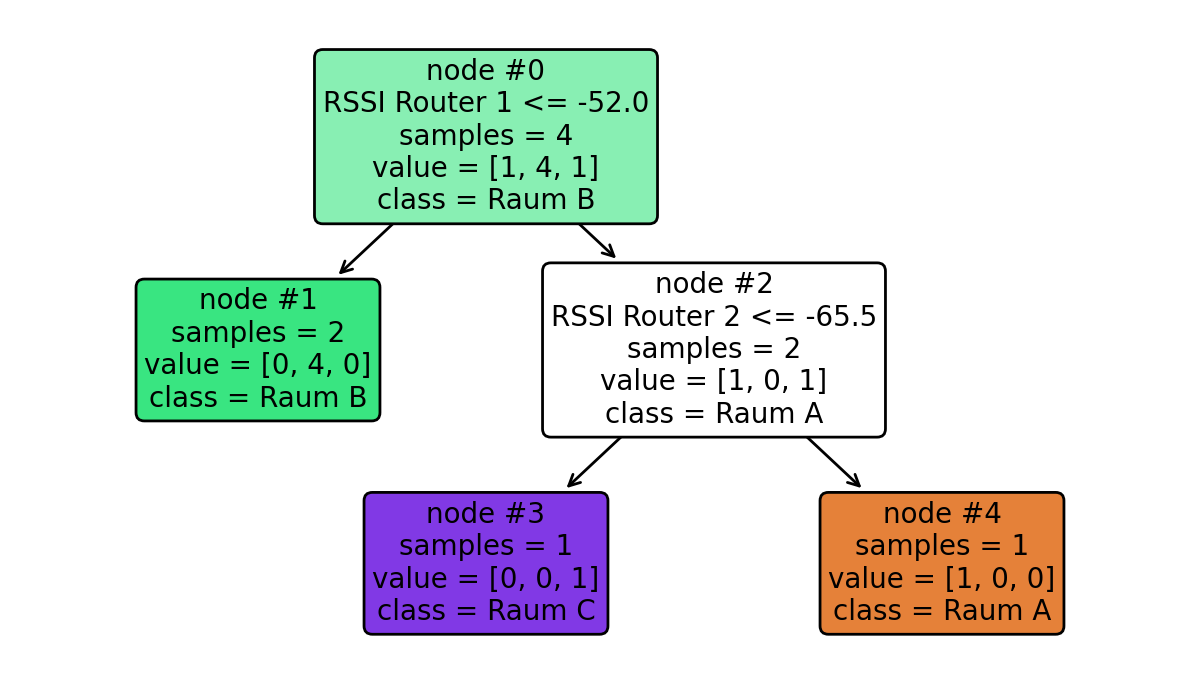
\includegraphics[width=0.4\textwidth]{images/random_forest.png}
    \caption{Darstellung eines Entscheidungsbaums anhand der Beispieldaten}
    \label{fig:random_forest}
\end{figure}


% \subsection{Parameter: Anzahl der Bäume (n\_estimators)}
